\documentclass[10pt]{beamer}
%% beamer template and options 
\mode<presentation>
{
  \usetheme{CambridgeUS}
  \usefonttheme{serif}
  \useoutertheme{default}
}\setbeamertemplate{navigation symbols}{} 



\usepackage[utf8]{inputenc}
\usepackage{xcolor,comment,cancel,tabularx,multirow}
\specialcomment{extended}{}{}    
\excludecomment{extended}
\usepackage{../styles/authordate1-4-beamer}

\usepackage{pgfplots}
\usepackage{xspace}
\usepackage{amsmath}
\usepackage{wasysym}
\usepackage{tikz}
\usetikzlibrary{automata,fit}
\usetikzlibrary{arrows}
\usetikzlibrary{shapes}
\usetikzlibrary{snakes}
\usetikzlibrary{arrows.meta,intersections}
\tikzstyle{every picture}+=[remember picture]
\usetikzlibrary{decorations.markings}





\title[IDL@BME-BIN] % (optional, use only with long paper titles)
{Introduction to Deep Learning} 
\subtitle{Sequence classification and modelling}

\author[A. Allauzen] % (optional, use only with lots of authors)
{Alexandre Allauzen}



\institute[ESPCI/Dauphine/PSL] % (optional, but mostly needed)
{
\includegraphics[height=3em]{../logos/espci_blue.png}\hfill
\raisebox{1.75ex}{\includegraphics[height=1.5em]{../logos/dauphine.png}}\\
\hfill\includegraphics[height=3em]{../logos/logomiles_white.pdf}
}




\date{12 and 13/10/20} % (optional)





\DeclareMathOperator*{\argmax}{argmax}
\DeclareMathOperator*{\argmin}{argmin}

\newcommand{\ngram}{\mbox{$n$-gram}\xspace} 



%% important : red + bf 
\def\important#1{{\bf \color{red} #1\/}}


%%% basics : 
\newcommand{\real}{\ensuremath{\mathbb{R}}}
\newcommand{\vct}[1]{\ensuremath{\mathbf{#1}}} % a vector / matrix is in bold
\newcommand{\seq}[1]{\ensuremath{\boldsymbol{#1}}}

\newcommand{\transp}[1]{\ensuremath{{#1}^{t} }} % transposition 
%\newcommand{\scal}[2]{\left\langle #1 , #2 \right\rangle} % scalair
%product
\newcommand{\scal}[2]{#1^t#2} % scalair product
\newcommand{\mydot}[2]{\ensuremath{ \transp{#1} #2}} % dot prod
\newcommand{\norm}[1]{\ensuremath{|| #1 ||}} % l2
\newcommand{\normabs}[1]{\ensuremath{ || #1 ||_{1} }} % l1




% vertical vector 
\newcommand{\vv}[1]{
	\left(
	\begin{array}[c]{c}
		#1 
	\end{array}
	\right)
}
% backeted vertical vector 
\newcommand{\vvb}[1]{
	\left[
	\begin{array}[c]{c}
		#1 
	\end{array}
	\right]
}
% raw vertical vector 
\newcommand{\vvr}[1]{
	\begin{array}[c]{c}
		#1 
	\end{array}
}





% words sequences sentences 
\newcommand{\ws}{{w}} % 
\newcommand{\wseq}{{\mathbf{\ws}}} % 
\newcommand{\length}{{L}} % 
\newcommand{\wsseq}[2]{{\ws_{#1}^{#2}}} % word subsequence
\newcommand{\word}[1]{{\it #1}} % an example
\newcommand{\vocab}{{\mathcal{V}}} % vocab

\newcommand{\asymb}{\ensuremath{a}} % symbol of *one* element of the
                                % alignment sequence
\newcommand{\ssymb}{\ensuremath{s}} % symbol of *one* element of the source
\newcommand{\tsymb}{\ensuremath{t}} % symbol of *one* element of the target


\newcommand{\aseq}{\ensuremath{\mathbf{\asymb}}} % alignment sentence
\newcommand{\sseq}{\ensuremath{\mathbf{\ssymb}}} % source sentence
\newcommand{\tseq}{\ensuremath{\mathbf{\tsymb}}} % target sentence


% misc 
\newcommand{\BigO}[1]{\ensuremath{\operatorname{O}\bigl(#1\bigr)}}
\newcommand{\bos}{\texttt{\textless s\textgreater}} 
\newcommand{\eos}{\texttt{\textless/s\textgreater}} 


% machine learning i/o and parameters ...
% params for model 
\newcommand{\param}{\ensuremath{\theta}} 
\newcommand{\params}{\ensuremath{\boldsymbol{\theta}}}
\newcommand{\nfeats}{\ensuremath{D}} % 

\newcommand{\x}{\ensuremath{\seq{x}}} % 
\newcommand{\X}{\ensuremath{\seq{X}}} % 
\newcommand{\y}{\ensuremath{\seq{y}}} % 
\newcommand{\z}{\ensuremath{\seq{z}}} % 
\newcommand{\w}{\ensuremath{\seq{w}}} % 
\newcommand{\pa}{\ensuremath{\seq{a}}} % 
\newcommand{\pb}{\ensuremath{\seq{b}}} % 

\newcommand{\W}{\seq{W}}
\newcommand{\V}{\seq{V}}
\newcommand{\pgrad}[1]{\nabla_{#1}}
\newcommand{\vgrad}[2]{\ensuremath{\nabla_{#1} #2}}

%%%%%%% data and loss
\newcommand{\nsamples}{\ensuremath{N}}
\newcommand{\ploss}{\ensuremath{l}} % for one datapoint
\newcommand{\class}{\ensuremath{{c}}} %
\newcommand{\rvclass}{\ensuremath{{C}}} %  the class as a RV 
\newcommand{\sid}[1]{\ensuremath{_{(#1)}}} % sample id
\newcommand{\tid}[1]{_{(#1)}} % time index for parameters
\newcommand{\exi}{\ensuremath{\x\sid{i}}} % 
\newcommand{\classi}{\ensuremath{\class\sid{i}}} % 
\newcommand{\nclasses}{\ensuremath{C}} % 
\newcommand{\yi}{y\sid{i}}  % prediction for sample i 

\newcommand{\dataset}{\ensuremath{\mathcal{D}}} % training data
\newcommand{\datax}{\ensuremath{\mathcal{X}}} % training data, x part
\newcommand{\datay}{\ensuremath{\tilde{\mathcal{Y}}}} % training data y part  
\newcommand{\datac}{\ensuremath{\tilde{\mathcal{C}}}} % training data c part (classes)
\newcommand{\ty}{\ensuremath{\tilde{y}}} % the supervised answer
\newcommand{\fullloss}{\ensuremath{\mathcal{L}(\params;\dataset)}}

%%% 
\newcommand{\nlaw}{\mathcal{N}}
\newcommand{\bern}{\ensuremath{\pi}}



%%%%%%%%%%%%%%%%%%%%%%%%%%%%%%%%%%%%%%%%%%%%%%%%%%%%%%%%%%%%
% a vector as a grid 
% 1: x 
% 2: y
% 3: the number of cells 
% The template :
% \node[rectangle,rounded corners,  draw, fill=red!20, text width=0.3*\textwidth, minimum height=6ex]  (label) at (0,0) {Hello} ;
\newcommand{\xvector}[3]{%
  \draw[step=.25] (#1-0.001,#2) grid (#1+0.25,#2+#3*0.25 );%
}

% notations 
% a layer l 
% input x^{(l)}
% output y^{(l)}
%  y^{(l)} = f^{(l)}( W^{(l)} input)
% note that 
% y_i = W_i,: x
% W_ij : x_j -> y_i  
% k is for the class
% l for the layer 


%%%%%%% to define layers math notations 
\newcommand{\inp}{\ensuremath{\x}}
\newcommand{\outp}{\ensuremath{\seq{y}}}
\newcommand{\lid}[1]{\ensuremath{^{(#1)}}}

%%%%%%% data and loss
\newcommand{\dlta}{\ensuremath{\delta}} % gradient component of pre-activation
\newcommand{\vdlta}{\ensuremath{\seq{\delta}}} % gradient vector of pre-activation

\colorlet{darkgreen}{green!50!black}


%% draw one layer 
\newcommand{\layer}{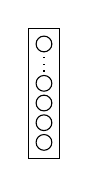
\begin{tikzpicture}[baseline=0.5ex]%
    \foreach \y in {0.25,0.5,...,1}{ 
      \draw (0,\y) circle  (0.1);%
    }
    \draw[dotted] (0.0, 1.15) -- (0.0,1.35); 
    \draw (0,1.5) circle (0.1);
    \draw (-0.2,0.05) rectangle (0.2,1.7);
\end{tikzpicture}}

%% draw connection
\newcommand{\connection}{\begin{tikzpicture}[baseline=0.5ex]%
    \draw[->] (0,0.85) -- (1.0,0.85);
\end{tikzpicture}}
%% dotted connection
\newcommand{\dotted}{\begin{tikzpicture}[baseline=0.5ex]%
    \draw[dotted,thick] (0,0.85) -- (0.5,0.85);%
\end{tikzpicture}}

\newcommand{\raiseW}{2ex}
% for computational graph
\newcommand{\vnode}{\node}
\newcommand{\funnode}{\node[minimum size=1.5,rectangle,draw=green,fill=green!20]}
\newcommand{\inlinefnode}[1]{\raisebox{-5pt}{\tikz{\funnode {#1}}}}



\newcommand{\justunder}{0.5cm}
\newcommand{\largeurUn}{0.8}
\newcommand{\largeurDeux}{0.7}
\setbeamercolor{postit}{fg=black,bg=red!30}
\setbeamercolor{mygreen}{fg=black,bg=green!20}
\setbeamercolor{myred}{fg=black,bg=red!20}
\setbeamercolor{darkpostit}{fg=black,bg=red!64}
\setbeamercolor{text}{fg=black,bg=red!10}


%%%%%%%%%% NNet for NLP
%% draw one layer  
\newcommand{\wemb}{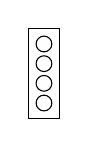
\begin{tikzpicture}[baseline=0.5ex]%
    \foreach \y in {0.25,0.5,...,1}{ 
      \draw (0,\y) circle  (0.1);%
    }
    \draw (-0.2,0.05) rectangle (0.2,1.2);
\end{tikzpicture}}

\newcommand{\worddim}{\ensuremath{K}} % dimension of the word embeddings
\newcommand{\wvector}{\ensuremath{\vct{v}}} % word vector
\newcommand{\wmatrix}{\ensuremath{\vct{R}}} % word matrix
\newcommand{\dvector}{\ensuremath{\vct{d}}} % document vector



%%%%%%%%% macro et redefinition 
\AtBeginSection[]
{
  \begin{frame}<beamer>
    \frametitle{Outline}
    \tableofcontents[currentsection]
  \end{frame}
}


\begin{document}
\tikzset{->-/.style={decoration={
  markings,
  mark=at position .5 with {\arrow{>}}},postaction={decorate}}}

\begin{frame}
  \titlepage
\end{frame}

\begin{frame}<beamer>
  \frametitle{Outline}
  \tableofcontents
\end{frame}
 






%%%%%%%%%%%%%%%%%%%%%%%%%%%%%%%%%%%%%%%%%%%%%%%%%%%%%%%%%%%%%%%%%%%%%%
\section{Introduction}
% examples
% - mnist
% - imdb
% - ARN / ADN 
% - NER (segmentation)
\begin{frame}{Image classification}
  \begin{center}
    \tikz[baseline=0]{ \node at (-2,0)
      {\includegraphics[height=0.25\textheight]{figs/mnist_5.pdf}}; %
      \node at (-0.4,0) {:}; \xvector{0}{-0.75}{6} }
    $\x \in \real^{784} \ \longrightarrow \class  \in\{0, 1,2, \ldots ,9
    \}$
  \end{center}
  \begin{itemize}
  \item $\dataset= (\exi , \classi )_{i=1}^{\nsamples}$ 
  \item \important{Supervised} learning of a \important{classification} task
  \end{itemize}
\end{frame}

\begin{frame}{Review classification}
  \begin{center}
    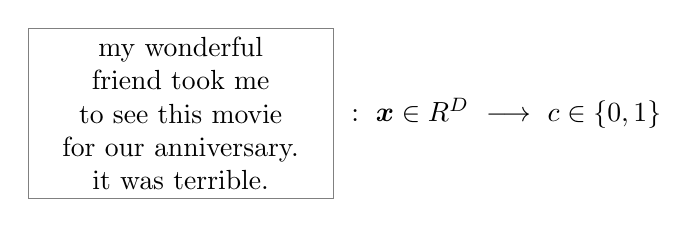
\begin{tikzpicture}
        %%%%%%%%%%%%%%%%%%%%%
      \node[anchor=east,draw=gray,text width=0.3\textwidth,align=center] (review) at
      (0,0) {my wonderful friend took me to see this movie \\for our
        anniversary. \\ it was terrible.};
      %%%%%%%%%%%%%%%%%%%%%
      \node[anchor=west] (txt) at (0.1,0) {$: \ \x \in \real^{\nfeats} \ \longrightarrow \ \class \in\{0, 1\}$};
    \end{tikzpicture}
  \end{center}

  \begin{itemize}
  \item $\dataset= (\exi , \classi )_{i=1}^{\nsamples}$ 
  \item The input is a sequence $\rightarrow$ how to build $\x$ ? 
  \item A sequence of words (discrete symbols)
  \item Words interact with each other, the neighborhood is important
  \end{itemize}
\end{frame}


%%%%%%%%%%%%%%%%%%%%%%%%%%%%%%%%%%%%%%%%%%%%%%%%%%%%%%%%%%%%%%%%%%%%%%%%%%%%%%%%%%%%
% https://en.wikipedia.org/wiki/Enhancer_(genetics)
% https://fr.wikipedia.org/wiki/Amplificateur_(biologie)
%
% In genetics, an enhancer is a short (50–1500 bp) region of DNA that
% can be bound by proteins (activators) t
%
% 3 articles :
% 2 on convNet 
% - https://www.ncbi.nlm.nih.gov/pmc/articles/PMC5773911/
% - https://www.biorxiv.org/content/10.1101/264200v2.full
% 1 on SVM k-mers
% https://www.ncbi.nlm.nih.gov/pubmed/21875935/
%%%%%%%%%%%%%%%%%%%%%%%%%%%%%%%%%%%%%%%%%%%%%%%%%%%%%%%%%%%%%%%%%%%%%%%%%%%%%%%%%%%%
% Alphabet = set of nucleotides: 
% A,C,G,T
\newcommand{\cga}{{\color{red!70!black} A}}
\newcommand{\cgc}{{\color{blue!70!black} C}}
\newcommand{\cgg}{{\color{yellow!70!black} G}}
\newcommand{\cgt}{{\color{green!70!black} T}}
\begin{frame}{Enhancer Identification in  DNA Sequences}
  \framesubtitle{From~\cite{Xu17Enhancer,Cohn18Enhancer}}
  \begin{quote}
    \small Enhancer sequences regulate the expression of genes from
    afar by providing a binding platform for transcription factors,
    (...). Despite
    their importance in health and disease, our understanding of these
    DNA sequences, and their regulatory grammar, is limited. This
    impairs our ability to identify new enhancers along the genome, or
    to understand the effect of enhancer mutations and their role in
    genetic diseases.
  \end{quote}
  \begin{block}{Sequence classification task / property identification}
    \begin{center}
      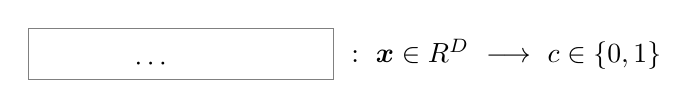
\begin{tikzpicture}
        %%%%%%%%%%%%%%%%%%%%% 
        \node[anchor=east,draw=gray,text width=0.3\textwidth,align=center] (review) at
        (0,0) {\cga~\cgt~\cgc~\cgg~\cga~\cgt~\cgc~\cgg\\$\cdots$~\cgg~\cgt~\cga~\cga~\cgt~\cgc~\cgg};
        %%%%%%%%%%%%%%%%%%%%% 
        \node[anchor=west] (txt) at (0.1,0) {$: \ \x \in \real^{\nfeats} \ \longrightarrow \ \class \in\{0, 1\}$};
      \end{tikzpicture}
    \end{center}
    \begin{itemize}
    \item Long sequence (arbitrary length)
    \item Only 4 discrete symbols, but  some subsequences are more informative (segments ?)
    \item Long range interactions between segments 
    \end{itemize}
  \end{block}
\end{frame}

\begin{frame}{Predicting the sequence specificities of DNA- and RNA-binding proteins}
  \framesubtitle{from \cite{Alipanahi15DNABinding}}
    \begin{quote}
      \small Knowing the sequence specificities of DNA- and
      RNA-binding proteins is essential for developing models of the
      regulatory processes in biological systems and for identifying
      causal disease variants.
  \end{quote}
  \begin{block}{Sequence classification / regression task}
    \begin{center}
      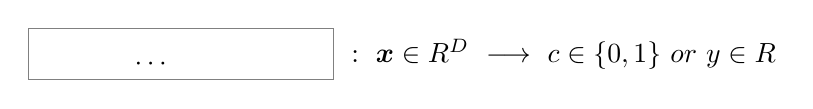
\begin{tikzpicture}
        %%%%%%%%%%%%%%%%%%%%%
        \node[anchor=east,draw=gray,text width=0.3\textwidth,align=center] (review) at
        (0,0) {\cga~\cgt~\cgc~\cgg~\cga~\cgt~\cgc~\cgg\\$\cdots$~\cgg~\cgt~\cga~\cga~\cgt~\cgc~\cgg};
        %%%%%%%%%%%%%%%%%%%%% 
        \node[anchor=west] (txt) at (0.1,0) {$: \ \x \in \real^{\nfeats} \ \longrightarrow \ \class \in\{0, 1\}\ or\ y \in \real$};
      \end{tikzpicture}
    \end{center}
    \begin{itemize}
    \item The data come in qualitatively different forms:
      \begin{itemize}
      \item Protein binding microarrays (PBMs) and RNAcompete assays
        provide a specificity coefficient for each probe sequence
      \item chromatin mmunoprecipitation (ChIP)-seq10 provides a
        ranked list of putatively bound sequences of varying length;
      \item HT-SELEX11 generates a set of very high affinity
        sequences.
    \end{itemize}
    \item Each  acquisition technology has its own artifacts, biases and limitations
    \end{itemize}
  \end{block}
\end{frame}



\begin{frame}{Audio classification / segmentation}
  \framesubtitle{\cite{Jang19Music}}
  \begin{center}
    \includegraphics[width=0.5\textwidth]{../figs/music_speech}    
  \end{center}
  \begin{itemize}
  \item Classification at each time step
  \item But the context is crucial (for the input and the output) ! 
  \end{itemize}
\end{frame}



\begin{frame}{Sequence generation}
  \begin{block}{Predicting the evolution of a dynamical system}
    \begin{columns}
      \column{0.5\textwidth}
      \begin{center}
        \includegraphics[width=\textwidth]{../figs/ks_h}
      \end{center}
      \column{0.5\textwidth}
      $$P(\y_{1:T}) = \prod_{i=1}^{T} P(\y_i | \y_{1:i-1})$$
    \end{columns}
  \end{block}
  \begin{block}{Sequence generation for sparse observation}
    \begin{columns}
      \column{0.5\textwidth}
      \begin{center}
        \includegraphics[width=\textwidth]{../figs/cylinder}
      \end{center}
      \column{0.5\textwidth}
      $$P(\y_{1:T}| \x ) = \prod_{i=1}^{T} P(\y_i | \y_{1:i-1}, \x)$$
    \end{columns}
  \end{block}
\end{frame}


\begin{frame}{Sequence tagging}
  \begin{align*}
   \wseq = \ws_{1}^{\length} &= \ws_1, \ws_2, ..., \ws_{\length}\\
   \tseq = \tsymb_{1}^{\length} &= \tsymb_1, \tsymb_2, ..., \tsymb_{\length}
  \end{align*}

  Example : Part-of-Speech (POS) tagging\\
  
  \begin{center}
    \begin{tabular}{l|l}
      Sentence &POS-tags\\\hline
      Er &PPER-case=nom$|$@gender=masc$|$number=sg$|$person=3\\
      fürchtet  &VVFIN-mood=ind$|$number=sg$|$person=3$|$tense=pres \\
      noch &ADV \\
      Schlimmeres &NN-case=acc$|$gender=neut$|$number=sg\\
      . &\$. 
    \end{tabular}
  \end{center}
\end{frame}


\newcolumntype{B}{>{\centering\arraybackslash} m{0.3\textwidth}}  %# New column type
\newcolumntype{C}{>{\centering\arraybackslash} m{0.25\textwidth}}  %# New column type
\begin{frame}{Speech recognition / Machine Translation}
    \begin{center}
    \begin{tabular}{B|C}
      \textit{Input} & \textit{Output}\\\hline
      \includegraphics[width=0.3\textwidth]{../figs/Signal-speech-martin-de.png} & $[$ Martine, boude $]$\\\hline\pause
      \multirow{3}{*}{$[$ il, est, temps $]$} & \multirow{3}{*}{$[$ es , ist , zeit $]$}   \\
      & \\
      &\\\hline\pause
      \multirow{3}{*}{$ \mathbf{x}  $} & \multirow{3}{*}{$\mathbf{y} = (y_1,  y_2, ... , y_I)$}  \\ & \\ & \\\hline
    \end{tabular}
  \end{center}\pause
    \begin{block}{\centering$P( \mathbf{y} | \mathbf{x}) = \prod_i^I P( y_i |\mathbf{y_{<i}},\mathbf{x}) $}
      \begin{itemize}
      \item Generate $\mathbf{y} $ from $\mathbf{x}$
      \item Evaluate $\mathbf{y}$ in the context $\mathbf{x}$
      \end{itemize}
    \end{block}
  % \begin{columns}
  %   \column{0.1\textwidth} 
  %   $$
  %   P( \mathbf{y} |  \mathbf{x}) \rightarrow
  %   $$
  %   \column{0.5\textwidth}
  %   \begin{itemize}
  %   \item Evaluate $\mathbf{y}$ in the context $\mathbf{x}$
  %   \item Generate $\mathbf{y} $ from $\mathbf{x}$
  %   \end{itemize}
  % \end{columns}
\end{frame}

\begin{frame}{Sequence in machine learning}
  \begin{block}{Sequence classification / regression}
    \begin{itemize}
    \item A sequence as input (of arbitrary length)
    \item Made of discrete symbols of real vectors 
    \item[$\rightarrow$] Predict a value, a class as output 
    \item[$\rightarrow$] Extract features from the sequence (summarize/compress)
    \item[$\rightarrow$] Represent the sequence as a whole to make a prediction
    \end{itemize}
  \end{block}
  \begin{block}{Generative sequence model}
    $$P( \mathbf{y} | \mathbf{x}) = \prod_i^I P( y_i |\mathbf{y_{<i}},\mathbf{x}) $$
  \end{block}
\end{frame}

\begin{frame}{Unsupervised pre-training and supervised fine-tuning}
  \begin{quote}
    Anotated datasets are usually scarce and sparse, while unannotated
    data are readily available
  \end{quote}
  \begin{block}{Unsupervised pre-training}
    Train a generative model of the input sequence: 
    $$P_{\params}( x_i |\mathbf{x_{<i}}) $$
    on unannotated data
  \end{block}
  \begin{block}{Supervised fine-tuning}
    Train a classifier $P_{\boldsymbol{\phi}} (\classi | \exi)$ on annotated dataset, but:
    \begin{itemize}
    \item Initialize some parameters (part of $\boldsymbol{\phi}$) with some parts of $\params$
    \item Optionally fine tune them. 
    \end{itemize}
  \end{block}

  
\end{frame}

\begin{frame}{DNA Sequence \textit{vs} Sentence classification}
  \begin{block}{Text representation}
    \begin{itemize}
    \item a text is a structured sequence made of words;
    \item a word is a discrete symbol;
    \item belonging to a \textit{finite} set: the vocabulary $\vocab$. 
    \end{itemize}
  \end{block}
  \begin{block}{Compositionality}
    \begin{itemize}
    \item {The meaning of a complex expression is determined by the
        meanings of its constituent,}
    \item {\color{red}and the rules used to combine them. }
    \end{itemize}
  \end{block}
  \begin{block}{DNA sequence}
    \begin{itemize}
    \item Potentially very long sequence made of 4 discrete symbols
    \item Subsequences can be compared to words, but the segmentation is missing
    \item Complexe interaction with long range dependancies 
    \end{itemize}
  \end{block}
\end{frame}

\endinput




%%%%%%%%%%%%%%%%%%%%%%%%%%%%%%%%%%%%%%%%%%%%%%%%%%%%%%%%%%%%%%%%%%%%%% 
\section{Neural Network language model}
\newcommand{\largeur}{0.5}
\newcommand{\hauteur}{1.5}
\newcommand{\rayon}{0.075cm}
\newcommand{\ytext}{-1}
\newcommand{\ytexth}{3*\hauteur+2.5}
\newcommand{\dlayer}[3]{ \draw[fill=#3] (#1,#2) rectangle (#1+\largeur,#2+\hauteur); %
  \foreach \y in {0.25,0.5,...,1.25}{ \draw[fill=black] (#1+\largeur/2,#2+\y) circle (\rayon);};%
}
\newcommand{\greenhc}{\color{green!50!black}}
\newcommand{\hiddenl}{\greenhc\seq{h}_t}



\newcommand{\wcontext}{\mathbf{h}}
\renewcommand{\mydot}[2]{\left\langle {#1} , {#2} \right\rangle} % scalair product

% \newcommand{gcolor}{red!40}
% \colorlet{gcolor}{green!60!black} % color for good word
\colorlet{gcolor}{blue} % color for good word
\colorlet{hcolor}{orange} % color for context 
\newcommand{\gw}{{\color{gcolor}\ws}} % good word
\newcommand{\gwi}{{\color{gcolor}\ws_i}} % good word
\newcommand{\whscore}{\ensuremath{s_{\params}({\gwi},{\color{hcolor}\wcontext})}}

\begin{frame}{A word prediction ``game''}
  \begin{center}
    $P( \ws_i = \textrm{?}  | \underbrace{\mathbf{\ws}_{1}^{i-1}
    }_{\color{orange}\textrm{context: }\mathbf{h}})\ \ \ \ \rightarrow\ \ \ $
    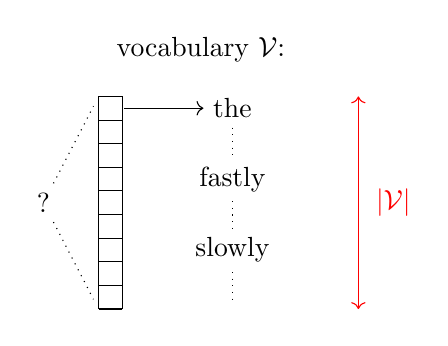
\begin{tikzpicture}[baseline=1.22cm]
      %%%%%%%%%%%%%%% 1st
      \node (pred) at (-1, 1.35) {?};

      { \node (the) at (1.4,2.55) {the}; }

      { \node (bas) at (-.3, 0) {}; \node (haut) at (-.3, 2.7) {};
        \draw[step=.3] (-.3, 0) grid (0, 2.7); \draw[dotted] (pred) --
        (bas); \draw[dotted] (pred) -- (haut);
        % 
        \node (voc) at (1,3.3) {vocabulary $\vocab$:}; \node (the0) at
        (-0.1,2.55) {};
        
        % 
        \node (fastly0) at (-0.1,1.65) {}; \node (fastly) at
        (1.4,1.65) {fastly}; \node (slowly0) at (-0.1,0.75) {}; \node
        (slowly) at (1.4,0.75) {slowly};

        \node (basmot) at (1.4,0) {}; \draw[->] (the0) -- (the);
        \draw[dotted] (the) -- (fastly); \draw[dotted] (fastly) --
        (slowly); \draw[dotted] (slowly) -- (basmot);

        \draw[<->,red] (3,2.7) -- (3,-0);
        \node[anchor=west,red] (V) at (3.1,1.35) {$|\vocab|$};
      }
    \end{tikzpicture}
  \end{center}
  \begin{itemize}
  \item $\vocab$ is a finite set of words 
  \item A probability distribution over $\vocab$, $\forall\
    {\color{orange}\mathbf{h}}$

  \item ${\color{orange}\mathbf{h}}=[\textrm{time}, \textrm{goes},
    \textrm{by}, \textrm{so} ]$
  \end{itemize}
\end{frame}


\begin{frame}
  \frametitle{Language model / Generative sequence model}
  \begin{block}{Applications}
    Automatic Speech Recognition, Machine Translation, OCR, ... 
  \end{block}

  \begin{block}{The goal}
    Estimate the \textbf{non-zero} probability of a word sequence given a vocabulary 
    $$
    P(\wsseq{1}{L}) = P(\ws_1, \ws_2, ... \ws_L) = \prod_{i=1}^L P(\ws_i | \wsseq{1}{i-1}),\ \ \forall i , \ws_i \in \vocab
    $$

    with the \textbf{\ngram assumption}:
    $$
    P(\wsseq{1}{L}) = \prod_{i=1}^L P(\ws_i | \wsseq{i-n+1}{i-1}),\ \ \forall i , \ws_i \in \vocab,
    $$

    in the \textbf{recurrent} way 
    $$ P(\ws_i | \wsseq{1}{i-1})$$
  \end{block}
\end{frame}


\begin{frame}{Challenges}
  \begin{itemize}
  \item Share knowledge among similar words
    \begin{center}
      \begin{tabular}{l|r}
        you {\color{red}go} to {\color{green}London} &you go to {\color{blue}Montelimar}\\
        you {\color{red}went} to {\color{green}London} &you went to {\color{blue}Montelimar}
      \end{tabular}
    \end{center}
  \item Keep/skip what is meaningful/meaningless
    \begin{center}
      Dr. Janet who visited us last year Smith talks about ...
    \end{center}
  \item Long distance dependancies
    \begin{center}
      to greatly play \textbf{chess} he wants to  have a nice \textbf{board}\\
      to greatly play \textbf{music} he wants to buy a new  \textbf{keyboard}
    \end{center}
  \end{itemize}
\end{frame}


\begin{frame}{Count-based language model}
  \framesubtitle{\ngram LM}
  \begin{align*}
    P(\wsseq{1}{L}) &= \prod_{i=1}^L P(\ws_i | \wsseq{i-n+1}{i-1}),\ \
                      \forall i , \ws_i \in \vocab,\\
    P_{ML}(\ws_i | \wsseq{i-n+1}{i-1}) &=
                                         \frac{c(\wsseq{i-n+1}{i})}{c(\wsseq{i-n+1}{i-1})}
  \end{align*}
  \begin{itemize}
  \item Very inefficient ! 
  \item How to deal with zero counts in the denominator ? 
  \item In the numerator ? 
  \item Zero counts are the most frequent case. 
  \item[$\rightarrow$] smoothing~\cite{Kneser95Improved,Chen98Empirical}
  \end{itemize}
\end{frame}


\begin{frame}{Estimate $n$-gram probabilities in a continuous space}
  Introduced in~\cite{Bengio01,Bengio03aneural} 
  \begin{block}{In a nutshell}
    \begin{enumerate}
    \item associate each word with a continuous feature vector
    \item express the probability function of a word sequence in terms
      of the feature vectors of these words
    \item learn simultaneously the feature vectors and the parameters
      of that probability function.
    \end{enumerate}
  \end{block}
  \begin{block}{Why should it work ?}
    \begin{itemize}
    \item  "similar" words are expected to have a similar feature vectors
    \item  the probability function is a smooth function of these
      feature values
      \begin{itemize}
      \item  a small change in the features will induce a small
        change in the probability
      \item Remember: \textsc{London} and \textsc{Montelimar}
      \end{itemize}
    \end{itemize}
  \end{block}
\end{frame}


\begin{frame}{Word (discrete symbols) embeddings}
  \begin{block}{One-hot encoding}
    \begin{center}
      \begin{displaymath}
        \textrm{Assume the vocabulary:~~~~~~~~~}
        \left.
          \begin{array}{l}
            the\\
            \mathbf{this}\\
            awesome\\
            ...\\
            great
          \end{array} 
        \right\} \rightarrow \x = 
        \left( 
          \begin{array}{c}
            0\\
            \mathbf{1}\\
            0\\
            ...\\
            0
          \end{array}
        \right)
      \end{displaymath}
    \end{center}
  \end{block}
  \begin{block}{Look-up table}
    \begin{center}
      \begin{displaymath} % 
        \underbrace{\wmatrix}_{\textrm{\tiny Look-up table}} \times \x = 
        \left(
          \begin{array}{ccccc}
            \vdots &\vdots &\vdots &\vdots &\vdots \\
            \wvector_{the} & \wvector_{this} & \wvector_{awesome} & \cdots &  \wvector_{great}\\
            \vdots &\vdots &\vdots &\vdots &\vdots \\
          \end{array} 
        \right) \times 
        \left( 
          \begin{array}{c}
            0\\
            \mathbf{1}\\
            0\\
            0\\
            0
          \end{array} 
        \right)  = \wvector_{this} 
      \end{displaymath}
    \end{center}
  \end{block}
\end{frame}


\begin{frame}
  \frametitle{Word embeddings}
  \begin{block}{Definitions}
    \begin{itemize}
    \item A continous vector associated to each word (discrete symbol): its
      \important{embedding}. 
    \item The matrix $\wmatrix$ is called the \important{look-up
        table} and store the word embeddings. 
    \end{itemize}
  \end{block}
  \begin{itemize}
  \item The term \textit{look-up} comes from the real operation\\
    $\wmatrix\times\x$ is only theoritical !
  \item No computational cost, only storage and trainability
    challenge\\ (enough observations for each words, ...) 
  \item Pre-trained, fine-tuned, ... 
  \end{itemize}
\end{frame}



\begin{frame}{Neural language model basics}
  \begin{columns}
    %%%%%%%%%%%%%%%%%%%%%%%%%%%%%%%%%%%%%%%%%%%%%%%%%%%%%%%%%%%% 
    \column{0.5\textwidth}
    \begin{center}
      \begin{tikzpicture}[scale=0.6,every node/.style={scale=0.7}]
        \node[anchor=mid] (time) at (0+\largeur/2,\ytext){$<$s$>$};
        \node[anchor=mid] (goes) at (2+\largeur/2,\ytext) {time};
        \node[anchor=mid] (by) at (4+\largeur/2,\ytext) {goes};
        \node[anchor=mid] (so) at (6+\largeur/2,\ytext) {by};
        \node[anchor=mid] (dots) at (8+\largeur/2,\ytext) {so};

        % words embeddings
        \uncover<2->{
          \foreach \x in {0,2,...,8}{\dlayer{\x}{0}{white}};
          % links from text to embeddings
          \foreach \x in {0,2,...,8}{\draw[->]
            (\x+\largeur/2,\ytext+0.2) -- (\x+\largeur/2,0);};

        }
        \uncover<3->{
          % links from embeddings to hidden layers
          \foreach \x in {0,2,...,8}{\draw
            (\x+\largeur/2,0+\hauteur) --
            (\x+\largeur/2,\hauteur+1);};
          % horizontal
          \draw (0+\largeur/2,\hauteur+1) --
          (8+\largeur/2,\hauteur+1);
          % merge arrow
          \draw[->] (4+\largeur/2,1+\hauteur) --
          (4+\largeur/2,\hauteur+2.5);
          % Composition operator
          \node[anchor=mid,fill=gray!20] (merge) at
          (4+\largeur/2,\hauteur+ 1.5)
          {\color{red}\large$\boldsymbol{\otimes}$};
          % Context vector
          \dlayer{4}{\hauteur+2.5}{hcolor}
        }
        \uncover<4->{
          % Output vector / embeddings
          \dlayer{5}{\hauteur+2.5}{gcolor}
          % output arrows
          \draw[-] (4+\largeur/2,2*\hauteur+2.5) --
          (4.5+\largeur/2,2*\hauteur+3) ;
          \draw[-] (5+\largeur/2,2*\hauteur+2.5) --
          (4.5+\largeur/2,2*\hauteur+3) ;
          \draw[->] (4.5+\largeur/2,2*\hauteur+3) --
          (4.5+\largeur/2,2*\hauteur+3.5) ;
          % output score
          \node[anchor=south] (s) at (4.5+\largeur/2,2*\hauteur+3.5)
          {$\whscore$};
        }
      \end{tikzpicture}
    \end{center}
    %%%%%%%%%%%%%%%%%%%%%%%%%%%%%%%%%%%%%%%%%%%%%%%%%%%%%%%%%%%% 
    \column{0.5\textwidth}
    \small
    To estimate $P(\gwi | \wsseq{1}{i-1})$:
    \begin{itemize}
    \item<2-> each $\ws_i \in \wsseq{1}{i-1} \rightarrow$ embedded
    \item<3-> build a context vector $\color{hcolor}\wcontext$ for $\wsseq{1}{i-1}$
    \item<4-> the score of  a target word $\gwi$:
      $$\whscore$$
    \end{itemize}
    \uncover<5->{\vspace{-4ex} Details:
      \begin{itemize}
      \item $\params$: all the parameters
      \item $\whscore=\mydot{\color{gcolor}\ws_i}{\color{hcolor}\wcontext} $
      \item The probability distribution: 
        \begin{align*}
          P(\ws_i | \wsseq{1}{i-1}) &= \frac{\exp(\whscore)}{Z({\color{hcolor}\wcontext})}\\
          Z({\color{hcolor}\wcontext}) &=  \sum_{\ws\in\vocab} \exp(s_{\params}(\ws,{\color{hcolor}\wcontext}))
        \end{align*}
      \item What is  {\color{red}\large$\boldsymbol{\otimes}$} ? 
      \end{itemize}
      \vfill
    }
    
  \end{columns}
\end{frame}



\begin{frame}{Estimate the $n$-gram probability}
  \begin{columns}
    \begin{column}{0.6\textwidth}
      % \begin{beamercolorbox}[center,rounded=true,sep=0.5ex]{postit}
      %   Estimate the \textit{n-gram} probability in terms of the
      %   sequence of feature vectors instead of multinomials
      % \end{beamercolorbox}\pause
      \begin{block}{The program}
        \begin{itemize}
          % \item Associate each word with feature vector
          %   in a continous space.\pause
        \item<1-> Given  the history expressed as a  feature vector :
          {$\mathbf{v}$} (only the $n-1$ last words)
        \item<2-> Create a feature vector for the next word: $$ \mathbf{h} = f(\mathbf{W}_{vh} \mathbf{v}) $$
        \item<3-> For all words given the history:
          \begin{align*}
            \mathbf{o} &= f(\mathbf{W}_{ho} \mathbf{h}) \\
            P(\ws_i|\wsseq{i-n+1}{i-1}) &= \frac{\exp(o_{w_i})}{\sum_{\ws
                                          \in \vocab}\exp(o_{w_i}) }
          \end{align*}
          % \item<4-> All the parameters must be learnt ($\mathbf{R}, \mathbf{W_{vh}}, \mathbf{W_{ho}} $)
        \end{itemize}
      \end{block}
    \end{column}
    \begin{column}{0.4\textwidth}
      % \only<1>{\includegraphics[height=0.8\textheight]{./figs/cslm_1.pdf}}
      \only<1|handout:0>{\includegraphics[width=\textwidth]{../figs/cslm_2.pdf}}
      \only<2|handout:0>{\includegraphics[width=\textwidth]{../figs/cslm_3.pdf}}
      \only<3-|handout:1>{\includegraphics[width=\textwidth]{../figs/cslm_4.pdf}}
    \end{column}
  \end{columns}
\end{frame}


\begin{frame}{Learning and inference issues}
  \begin{block}{Training objective and gradients}
    \begin{align*}
      \fullloss &=  \sum_{(\ws,\wcontext) \in \dataset}  \log P_{\params}(\ws|\wcontext) \\
      \frac{\partial\fullloss }{ \partial\params} &=  \frac{\partial  \whscore} {\partial \params} - \sum_{\ws'\in\vocab} P_{\params}(\ws'|\wcontext)  \frac{ \partial  s_{\params}(\ws',\wcontext)}{\partial \params}
    \end{align*}
    % The vocabulary size $|\vocab| \Rightarrow$
    \begin{itemize}
    \item Large $|\vocab|$ is prohibitive
    \item Prediction in a high dimensional space
    \end{itemize}
  \end{block}
  \begin{block}{Solutions}
    \begin{itemize}
    \item Structured output~\cite{Le10Training,Le11Soul,Le13SOUL}
    \item New training criterion~\cite{Mnih12Fast,labeau17NCE}
    \end{itemize}
  \end{block}
\end{frame}




%%%%%%%%%%%%%%%%%%%%%%%%%%%%%%%%%%%%%%%%%%%%%%%%%%%%%%%%%%%%%%%%%%%%%% 
\section{Case study: ADN sequence classification}
\begin{frame}{Problem setting}
    \begin{block}{Sequence classification task / property identification}
    \begin{center}
      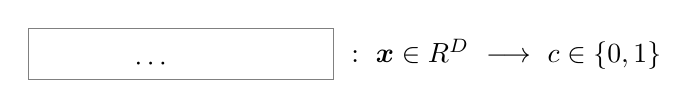
\begin{tikzpicture}
        %%%%%%%%%%%%%%%%%%%%% 
        \node[anchor=east,draw=gray,text width=0.3\textwidth,align=center] (review) at
        (0,0) {\cga~\cgt~\cgc~\cgg~\cga~\cgt~\cgt~\cgc\\$\cdots$~\cgg~\cgt~\cga~\cga~\cgt~\cgc~\cgg};
        %%%%%%%%%%%%%%%%%%%%% 
        \node[anchor=west] (txt) at (0.1,0) {$: \ \x \in \real^{\nfeats} \ \longrightarrow \ \class \in\{0, 1\}$};
      \end{tikzpicture}
      $$\dataset= (\seq{s}\sid{i} , \classi )_{i=1}^{\nsamples}$$ 
    \end{center}
  \end{block}
  \begin{block}{Classification assumption}
    \begin{itemize}
    \item The input $\seq{s}\sid{i}$ can be "summarized" in a vector $\exi$ 
    \item The classification is performed by a linear classification (layer)
    \item The loss can be the binary cross entropy 
    \item How can we process and transform $\seq{s}\sid{i}$ to build  $\exi$ ? 
    \end{itemize}
  \end{block}
\end{frame}


\begin{frame}{Feature engineering}
  \framesubtitle{Count based summarization / bag of features}
  \begin{center}
    \cga~\cgt~\cgc~\cgg~\cga~\cgt~\cgc~\cgg~\cgg~\cgt~\cga~\cga~\cgt~\cgc~\cgg
  \end{center}
  \begin{columns}
    \column{0.25\textwidth}
    \begin{center}
      \begin{tabular}{l|c}
        $\vocab$  &count    \\\hline
        \cga    &4 \\
        \cgc    &3 \\
        \cgg    &4 \\
        \cgt    &4 \\\hline
      \end{tabular}
    \end{center}\pause
    \column{0.1\textwidth}
    {\Large$$+$$}
    \column{0.25\textwidth}
    \begin{center}
      \begin{tabular}{l|c}
        ...$\vocab$  &count    \\\hline
        \cga \cga    &1 \\
        \cga \cgc    &0 \\
        \cga \cgg    &0 \\
        \cga \cgt    &3 \\\hline
        \cgc \cga    &0 \\
        \cgc \cgc    &0 \\
        \cgc \cgg    &1 \\
        \cgc \cgt    &0 \\\hline
      \end{tabular}
    \end{center}
    \column{0.1\textwidth}
    {\Large$$+$$}
    \column{0.25\textwidth}
    \begin{center}
      \begin{tabular}{l|c}
        ...$\vocab$  &count    \\\hline
        \cgg \cga    &1 \\
        \cgg \cgc    &0 \\
        \cgg \cgg    &1 \\
        \cgg \cgt    &0 \\\hline
        \cgt \cga    &1 \\
        \cgt \cgc    &3 \\
        \cgt \cgg    &0 \\
        \cgt \cgt    &0 \\\hline
      \end{tabular}
    \end{center}
  \end{columns}
  \begin{center}
    $\Rightarrow \x$ of dimension $m+m^2$, with $m$ the number of symbols
  \end{center}
\end{frame}

\begin{frame}{$k$-mers representation (\textit{aka} $n$-grams)}
  \framesubtitle{From \cite{Lee11DNA}}
   a $k$-mers are oligomers of length $k$
  \begin{block}{Transform $\seq{s}$ to $\x$ with $k$-mers encoding}
    \begin{itemize}
    \item Count the  set of $k$-mers of varying length (3–10 bp) in $\seq{s}$
    \item Generate a vector of $d$ dimensions
      $$
      \nfeats =  4^4 + 4^5 + 4^6 + 4^7 + 4^8 + 4^9 + 1 (\textrm{for padding}) =  349441
      $$
    \end{itemize}
  \end{block}
  \begin{block}{Linear (or not) classifier (SVM) }
    The model is parametrized with $\w$:
    $$
    \scal{\w}{\x} = \sum_{j=0}^{\nfeats} \underbrace{\color{red}w_j}_{\color{red}\textrm{representation of the oligomer}} \times \underbrace{\color{green!70!black}x_j}_{\color{green!70!black}\textrm{its count}}
    $$
  \end{block}
\end{frame}

\begin{frame}{ADN sequence classifier}
  The goal is to design a way to represent the sequence as a vector:
%  \begin{block}{Subsequence of discrete symbols}
    \begin{itemize}
    \item The oligomer $j$ is represented by  $w_j$: its contribution to the decision
    \item each oligomer of length $k$ is considered as a discrete symbol
    \item As $k$ increases, observations are sparse
    \item No interaction between oligomers (except the value of $w_j$):
      % CATTGTYATGCAAAT
      % \cgc\cga\cgt\cgt\cgg\cgt\cgy\cga\cgt\cgg\cgc\cga\cga\cga\cgt
      \begin{center}
      \begin{tabular}{llllr}
        \cgc&\cga&\cgt\cgt\cgg\cgt&     &$\rightarrow$ 1.45\\
            &\cga&\cgt\cgt\cgg\cgt&\cgc &$\rightarrow$ 1.19\\
        \cgc&\cgt&\cgt\cgt\cgg\cgt&     &$\rightarrow$ 1.06
      \end{tabular}
    \end{center}
  \item The count summarizes its contribution.
  \end{itemize}
 % \end{block}
  \begin{block}{Roadmap}
    \begin{itemize}
    \item Symbol embeddings
    \item Convolution 
    \item Pooling
    \end{itemize}
  \end{block}
\end{frame}

%%%%%%%%%%%%%%%%%%%%%%%%%%%%%%%%%%%%%%%%%%%%%%%%%%%%%%%%%%%%%%%%%%%%%%
\section{Sequence classification with convolution NNet}
%%%%%%%%%%%%%%%%%%%%%%%%%%%%%%%%%%%%%%%%%%%%%%%%%%%%%%%%%%%%%%%%%%
\begin{frame}{Another view of a sequence}
    \begin{center}
      \begin{displaymath}
          \begin{array}{lcccccccc}
            \seq{s}=&[ &\cgc&\cga&\cgt&\cgt&\cgg&\cgt
                        &]\\
            &&\downarrow &\downarrow &\downarrow &\downarrow &\downarrow &\downarrow \\
            \textrm{Look-up}&&\wemb &\wemb &\wemb &\wemb &\wemb &\wemb  \\
               &&\wvector_{\cgc}&\wvector_{\cga}&\wvector_{\cgt}&\wvector_{\cgt}&\wvector_{\cgg}&\wvector_{\cgt} \\
          \end{array}
        \end{displaymath}
        {\huge $\downarrow$} \\
        \tikz{\draw[step=0.5,black,thin] (0,0) grid (3,2);}
    \end{center}
\end{frame}



%%%%%%%%%%%%%%%%%%%%%%%%%%%%%%%%%%%%%%%%%%%%%
\begin{frame}
  \frametitle{Inspiration}
  \begin{block}{Convolutional Neural Networks for Sentence
      Classification}
    \begin{itemize}
    \item A short paper of 2014~\cite{Kim14Convolution}
    \item A simple and SOTA paper on text classification
    \end{itemize}
  \end{block}
  \begin{block}{Highlights}
    \begin{columns}
      \column{0.3\textwidth}{
        \begin{center}
          $\x$\\[1ex]
          {\huge $\downarrow$} \\[1ex]
          \tikz{\draw[step=0.5,black,thin] (0,0) grid (3,2);}
      \end{center}
    }
    %%%%
    \column{0.7\textwidth}{%
      \begin{itemize}
      \item This input matrix is a sequence of vectors 
      \item We can extract features with convolution filters
      \item The filters and the embeddings are parameters \\(to be learnt)
      \end{itemize}
    }
    \end{columns}
  \end{block}
  Application to DNA classification in~\cite{Xu17Enhancer,Cohn18Enhancer}
\end{frame}


%%%%%%%%%%%%%%%%%%%%%%%%%%%%%%%%%%%%%%%%%%%%%%%%%%%%%%%%%%%%%%%%%%
% In pytorch the indices are :
% batch, channel, data-point
% The data point for a 1D input is (t,d)
% For an image it is (x,y)
\begin{frame}{Convolution 1D}
  \framesubtitle{Extract a frame, or a window, and apply a ``filter''}
  \begin{columns}
    \column{0.6\textwidth}
    %%% the input : a matrix + window
    \begin{center}
    The input sequence of  $L=6$ \\vectors in $\real^{\nfeats}$,  $\nfeats=4$ \\[1ex]
    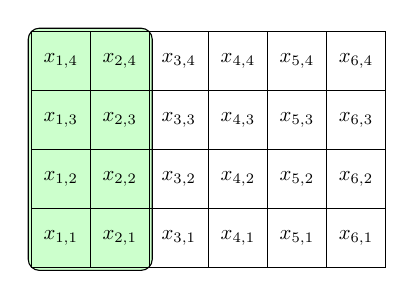
\begin{tikzpicture}[scale=0.75,every node/.style={scale=0.75}]
      % the window
      % offset for x and y of .5 + a bit more 
      \draw[fill=green!20,rounded corners] (0.45,0.45) rectangle (2.55,4.55); % green 
      %% the grid 
      \foreach \l in {1,2,...,4}
      \foreach \c in {1,2,...,6}
      {
        \draw (\c,\l) +(-.5,-.5) rectangle ++(.5,.5);
        \draw (\c,\l) node{$x_{\c,\l}$};
      }
    \end{tikzpicture}
  \end{center}
    \column{0.6\textwidth}
    \begin{center}
    The filter:\\kernel size of $ks=2$\\[1ex]
    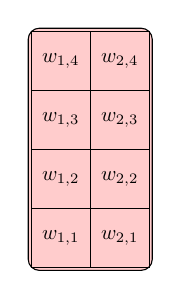
\begin{tikzpicture}[scale=0.75,every node/.style={scale=0.75}]
      % the window
      % offset for x and y of .5 + a bit more 
      \draw[fill=red!20,rounded corners] (0.45,0.45) rectangle (2.55,4.55); % green 
      
      %% the grid 
      \foreach \l in {1,2,...,4}
      \foreach \c in {1,2}
      {
        \draw (\c,\l) +(-.5,-.5) rectangle ++(.5,.5);
        \draw (\c,\l) node{$w_{\c,\l}$};
      }
    \end{tikzpicture}
  \end{center}
\end{columns}
\begin{block}{The output value (output channel)}
  $$
  \textrm{At time }t = 1,\ {\color{red!70!black} h_1} = \sum_{i,j} {\color{red!70!black}w_{i,j}}\times  {\color{green!70!black}x_{i,j}}
  $$
\end{block}
\end{frame}


%%%%%%%%%%%%%%%%%%%%%%%%%%%%%%%%%%%%%%%%%%%%%%%%%%%%%%%%%%%%%%%%%%%%%%%%%%%
\newcommand{\xs}{4}
\newcommand{\ys}{-4}
\begin{frame}{Convolution 1D: sliding along one dimension}
  \framesubtitle{Stride, or a sliding window}
  The input  is a matrix $(L=6,d=4)$, one filter of kernel size $=2$:~\\[1ex]
  \begin{block}{With a stride $= 1$}
    \begin{tikzpicture}[scale=0.5]
      %% the grid 
      \draw[step=0.5,black,thin] (0,0) grid (3,2);
      %%%%%%% 1 
      \draw[fill=red] (0+\xs,0) rectangle (1+\xs,2); % red 
      \draw[step=0.5,black,thin] (0+\xs,0) grid (3+\xs,2); % grid
      \draw[step=0.5,red] (-0.01+\xs,-0.5) grid (0.5+\xs,-1);    % grid res
      % arrow
      \draw[->,red]   (0.25+\xs,0) --  (0.25+\xs,-0.5);
      %%%%%%% 2 
      \draw[fill=red] (0.5+2*\xs,0) rectangle (1.5+2*\xs,2); % red 
      \draw[step=0.5,black,thin] (-0.01+2*\xs,0) grid (3+2*\xs,2); % grid
      \draw[step=0.5,red] (-0.01+2*\xs,-0.5) grid (1+2*\xs,-1);    % grid res
      % arrow
      \draw[->,red]   (0.75+2*\xs,0) --  (0.75+2*\xs,-0.5);

      %%%%%%% 3 
      \draw[fill=red] (0.99+3*\xs,0) rectangle (2+3*\xs,2); % red 
      \draw[step=0.5,black,thin] (-0.01+3*\xs,0) grid (3+3*\xs,2); % grid
      \draw[step=0.5,red] (-0.01+3*\xs,-0.5) grid (1.5+3*\xs,-1);    % grid res
      % arrow
      \draw[->,red]   (1.25+3*\xs,0) --  (1.25+3*\xs,-0.5);

      %%%%%%% 4
      \draw[fill=red] (1.49+4*\xs,0) rectangle (2.5+4*\xs,2); % red 
      \draw[step=0.5,black,thin] (-0.01+4*\xs,0) grid (3+4*\xs,2); % grid
      \draw[step=0.5,red] (-0.01+4*\xs,-0.5) grid (2+4*\xs,-1);    % grid res
      % arrow
      \draw[->,red]   (1.75+4*\xs,0) --  (1.75+4*\xs,-0.5);

      %%%%%%% 5 
      \draw[fill=red] (1.99+5*\xs,0) rectangle (3+5*\xs,2); % red 
      \draw[step=0.5,black,thin] (-0.01+5*\xs,0) grid (3+5*\xs,2); % grid
      \draw[step=0.5,red] (-0.01+5*\xs,-0.5) grid (2.5+5*\xs,-1);    % grid res
      % arrow
      \draw[->,red]   (2.25+5*\xs,0) --  (2.25+5*\xs,-0.5);
    \end{tikzpicture}
  \end{block}
  \begin{block}{With a stride = 2}
    \begin{tikzpicture}[scale=0.5]
      %% the grid 
      \draw[step=0.5,black,thin] (0,0) grid (3,2);
      %%%%%%% 1 
      \draw[fill=red] (0+\xs,0) rectangle (1+\xs,2); % red 
      \draw[step=0.5,black,thin] (0+\xs,0) grid (3+\xs,2); % grid
      \draw[step=0.5,red] (-0.01+\xs,-0.5) grid (0.5+\xs,-1);    % grid res
      \draw[->,red]   (0.25+\xs,0) --  (0.25+\xs,-0.5);       % arrow

      %%%%%%% 3 
      \draw[fill=red] (0.99+3*\xs,0) rectangle (2+3*\xs,2); % red 
      \draw[step=0.5,black,thin] (-0.01+3*\xs,0) grid (3+3*\xs,2); % grid
      \draw[step=0.5,red] (-0.01+3*\xs,-0.5) grid (0.5+3*\xs,-1);    % grid res
      \draw[step=0.5,red] (-0.01+3*\xs+1,-0.5) grid (1.5+3*\xs,-1);    % grid res
      % arrow
      \draw[->,red]   (1.25+3*\xs,0) --  (1.25+3*\xs,-0.5);
      %%%%%%% 5 
      \draw[fill=red] (1.99+5*\xs,0) rectangle (3+5*\xs,2); % red 
      \draw[step=0.5,black,thin] (-0.01+5*\xs,0) grid (3+5*\xs,2); % grid
      \draw[step=0.5,red] (-0.01+5*\xs,-0.5) grid (0.5+5*\xs,-1);    % grid res
      \draw[step=0.5,red] (-0.01+5*\xs+1,-0.5) grid (1.5+5*\xs,-1);    % grid res
      \draw[step=0.5,red] (-0.01+5*\xs+2,-0.5) grid (2.5+5*\xs,-1);    % grid res
      % arrow
      \draw[->,red]   (2.25+5*\xs,0) --  (2.25+5*\xs,-0.5);
    \end{tikzpicture}
  \end{block}
\end{frame}


%%%%%%%%%%%%%%%%%%%%%%%%%%%%%%%%%%%%%%%%%%%%%%%%%%%%%%%%%%%%%%%%%%%%%%%%%%%%%%%%%%%%%%%% 
\begin{frame}{Convolution 1D}
  \framesubtitle{With 2 output channels}
  \begin{columns}
    \column{0.6\textwidth}
    %%% the input : a matrix + window
    \begin{center}
      $L=6$,  $\nfeats=4$ \\[1ex]
      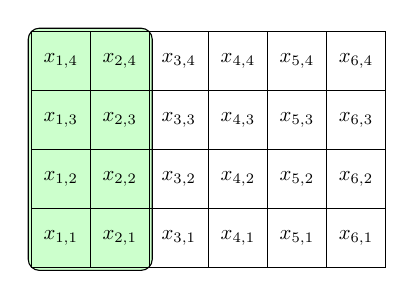
\begin{tikzpicture}[scale=0.75,every node/.style={scale=0.75}]
        % the window
        % offset for x and y of .5 + a bit more 
        \draw[fill=green!20,rounded corners] (0.45,0.45) rectangle (2.55,4.55); % green 
        %% the grid 
        \foreach \l in {1,2,...,4}
        \foreach \c in {1,2,...,6}
        {
          \draw (\c,\l) +(-.5,-.5) rectangle ++(.5,.5);
          \draw (\c,\l) node{$x_{\c,\l}$};
        }
      \end{tikzpicture}
    \end{center}
    \column{0.4\textwidth}
    \begin{center}
      Filters:kernel size of $ks=2$\\[1ex]
      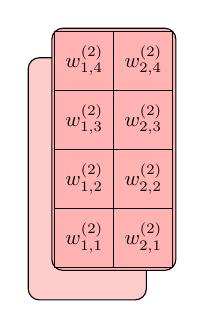
\begin{tikzpicture}[scale=0.75,every node/.style={scale=0.75}]
        % the window
        % offset for x and y of .5 + a bit more 
        \draw[fill=red!20,rounded corners] (0.05,-0.05) rectangle (2.05,4.05); % first 
        \draw[fill=red!30,rounded corners] (0.45,0.45) rectangle (2.55,4.55); 
        %% the grid 
        \foreach \l in {1,2,...,4}
        \foreach \c in {1,2}
        {
          \draw (\c,\l) +(-.5,-.5) rectangle ++(.5,.5);
          \draw (\c,\l) node{$w_{\c,\l}\lid{2}$};
        }
      \end{tikzpicture}
    \end{center}
  \end{columns}
  \begin{block}{The output value (output channel)}
    \begin{align*}
      {\color{red!70!black} h_{1,1}} &= \sum_{i,j} {\color{red!70!black}w_{i,j}\lid{1}}\times  {\color{green!70!black}x_{i,j}} \\
      {\color{red!70!black} h_{2,1}} &= \sum_{i,j} {\color{red!70!black}w_{i,j}\lid{2}}\times  {\color{green!70!black}x_{i,j}} 
    \end{align*}
  \end{block}
\end{frame}



%%%%%%%%%%%%%%%%%%%%%%%%%%%%%%%%%%%%%%%%%%%%%%%%%%%%%%%%%%%%%%%%%%%%%%%%%%%%%%%%%%%%%%%% 
\begin{frame}{Another wiew for two output channels}
  \begin{columns}
    \column{0.5\textwidth}
    \begin{tikzpicture}[scale=0.8]
      %%%%%%% the sentence as a matrix
    \draw[fill=green!20] (0,0) rectangle (0.5,2); % red 
    \draw[fill=green!60] (0.5,0) rectangle (1,2); % red 
    \draw[step=0.5,black,thin] (0,0) grid (3,2); % grid
    %%%%% window extract 
    \draw[fill=green!60] (0,-1+\ys) rectangle (0.5,1+\ys); % red
    \draw[fill=green!20] (0,1+\ys) rectangle (0.5,3+\ys); % red
    \draw[step=0.5,black,thin] (0,-1+\ys) grid (0.5,3+\ys); % grid
    %%%  
    \draw[->,red] (0.25,0) -- (0.25,-1); % arrow
    %%% Filter 
    \node (times) at (1,1+\ys) {$\rightarrow$};
    \draw[fill=red!60] (1.49,0.5+\ys) rectangle (1.5+4,1+\ys); % colors
    \draw[fill=red!30] (1.49,1+\ys) rectangle (1.5+4,1.5+\ys); % colors 
    \draw[step=0.5,black] (1.49,0.5+\ys) grid (1.5+4,1.5+\ys); % grid
    \node (times) at (4,-0.5+\ys) {$\W$};
    %%%
    \draw[->,red] (5.8,1+\ys) -- (6.8,1+\ys); % arrow
    \draw[fill=red!60] (7-0.01,0.5+\ys) rectangle (7.5,1+\ys); % grid
    \draw[fill=red!30] (7-0.01,1+\ys) rectangle (7.5,1.5+\ys); % grid
    \draw[step=0.5,thin] (7-0.01,0.5+\ys) grid (7.5,1.5+\ys); % grid
  \end{tikzpicture}
  \column{0.5\textwidth}
  \begin{itemize}
  \item {\color{red!30!black} Two filters } applied to the same {\color{green!30!black} frame (or window)}
  \item Each filter generates one feature 
  \item[$\rightarrow$]  a vector of two values, two features $( h_{1,1},  h_{2,1})$
  \item $ h_{c,t}$ is the feature extracted for the channel $c$ at time $t$. 
  \item $\W$ gathers the parameters of the filters in one matrix
  \item The parameters $\W$ are learnt
  \end{itemize}
\end{columns}

\end{frame}



%%%%%%%%%%%%%%%%%%%%%%%%%%%%%%%%%%%%%%%%%%%%%%%%%%%%%%%%%%%%%%%%%%%%%%%%%%%%%%%%%%%%%%%% 
\begin{frame}
  \frametitle{1D-convolution and pooling}
  The input text is a matrix $(L=6,d=4,od=2)$ after the embedding step:~\\[1ex]
  \begin{tikzpicture}[scale=0.5]
    %% the grid 
    \draw[step=0.5,black,thin] (0,0) grid (3,2);
  %%%%%%% 1 
    \draw[fill=red] (0+\xs,0) rectangle (1+\xs,2); % red 
    \draw[step=0.5,black,thin] (0+\xs,0) grid (3+\xs,2); % grid
    \draw[step=0.5,red] (-0.01+\xs,-0.5) grid (0.5+\xs,-1.5);    % grid res
    % arrow
    \draw[->,red]   (0.25+\xs,0) --  (0.25+\xs,-0.5);
  %%%%%%% 2 
    \draw[fill=red] (0.5+2*\xs,0) rectangle (1.5+2*\xs,2); % red 
    \draw[step=0.5,black,thin] (-0.01+2*\xs,0) grid (3+2*\xs,2); % grid
    %grid res
    \draw[step=0.5,red] (-0.01+2*\xs,-0.5) grid (1+2*\xs,-1.5);    % grid res
    % arrow
    \draw[->,red]   (0.75+2*\xs,0) --  (0.75+2*\xs,-0.5);

  %%%%%%% 3 
    \draw[fill=red] (0.99+3*\xs,0) rectangle (2+3*\xs,2); % red 
    \draw[step=0.5,black,thin] (-0.01+3*\xs,0) grid (3+3*\xs,2); % grid
    \draw[step=0.5,red] (-0.01+3*\xs,-0.5) grid (1.5+3*\xs,-1.5);    % grid res
    % arrow
    \draw[->,red]   (1.25+3*\xs,0) --  (1.25+3*\xs,-0.5);

  %%%%%%% 4
    \draw[fill=red] (1.49+4*\xs,0) rectangle (2.5+4*\xs,2); % red 
    \draw[step=0.5,black,thin] (-0.01+4*\xs,0) grid (3+4*\xs,2); % grid
    \draw[step=0.5,red] (-0.01+4*\xs,-0.5) grid (2+4*\xs,-1.5);    % grid res
    % arrow
    \draw[->,red]   (1.75+4*\xs,0) --  (1.75+4*\xs,-0.5);

  %%%%%%% 5 
    \draw[fill=red] (1.99+5*\xs,0) rectangle (3+5*\xs,2); % red 
    \draw[step=0.5,black,thin] (-0.01+5*\xs,0) grid (3+5*\xs,2); % grid
    \draw[step=0.5,red] (-0.01+5*\xs,-0.5) grid (2.5+5*\xs,-1.5);    % grid res
    % arrow
    \draw[->,red]   (2.25+5*\xs,0) --  (2.25+5*\xs,-0.5);

  \end{tikzpicture}\\[1ex]\vfill
  %%
  \begin{itemize}
  \item The transformation:  a matrix of size $(od, ws\times d)=(2, 8)$
  \item $ws$: window size
  \item $od$ is sometime called the number of featuremap. 
  \end{itemize}
  \begin{block}{Max-pooling over-time}
  \begin{center}
    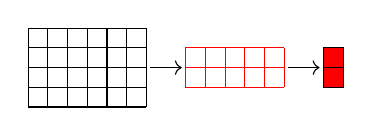
\begin{tikzpicture}[scale=0.5]
      %% the grid
      \draw[step=0.5,black,thin] (0,0) grid (3,2);
      \draw[->] (3.1,1)-- (3.9,1);
      \draw[step=0.5,red,thin] (3.99,0.5) grid (6.5,1.5);
      \draw[->] (6.6,1)-- (7.4,1);
      
      %%%%%%% final
      \draw[fill=red] (7.5,0.5) rectangle  (8,1.5); 
      \draw[step=0.5,black] (7.5,0.5) grid (8,1.5); % grid res
    \end{tikzpicture}
  \end{center}
\end{block}

\end{frame}



%%%%%%%%%%%%%%%%%%%%%%%%%%%%%%%%%%%%%%%%%%%%%%%%%%%%%%%%%%%%%%%%%%%%%%%%%%%%%%%%%%%%%%%% 
\renewcommand{\xs}{5}
\begin{frame}
  \frametitle{More Convolutions}
  \begin{center}
  The window size can vary: \\[3ex]
  \begin{tikzpicture}[scale=0.5]
    %%%%%  for 2 
    \draw[fill=red] (1.99+0*\xs,0) rectangle (3+0*\xs,2); % red 
    \draw[step=0.5,black,thin] (-0.01+0*\xs,0) grid (3+0*\xs,2); % grid
    \draw[step=0.5,red] (-0.01+0*\xs,-0.5) grid (2.5+0*\xs,-1.5);    % grid res
    \draw[fill=red] (2.5-0.01+0*\xs,-0.5) rectangle (3+0*\xs,-1.5);    % polling
    \draw[step=0.5,black] (2.5-0.01+0*\xs,-0.5) grid (3+0*\xs,-1.5);    % pooling

    %% the grid for 3 
    \draw[fill=green] (1.5+1*\xs,0) rectangle (3+1*\xs,2); % green
    \draw[step=0.5,black,thin] (0-0.01+1*\xs,0) grid (3+1*\xs,2);
    \draw[step=0.5,green] (-0.01+1*\xs,-0.5) grid (2+1*\xs,-1.5);    % grid res
    \draw[fill=green] (2.5-0.01+1*\xs,-0.5) rectangle (3+1*\xs,-1.5);    % polling
    \draw[step=0.5,black] (2.5-0.01+1*\xs,-0.5) grid (3+1*\xs,-1.5);    % pooling

    %% the grid for 4
    \draw[fill=blue] (1+2*\xs,0) rectangle (3+2*\xs,2); % blue
    \draw[step=0.5,black,thin] (0-0.01+2*\xs,0) grid (3+2*\xs,2);
    \draw[step=0.5,blue] (-0.01+2*\xs,-0.5) grid (1.5+2*\xs,-1.5);    % grid res
    \draw[fill=blue] (2.5-0.01+2*\xs,-0.5) rectangle (3+2*\xs,-1.5);    % polling
    \draw[step=0.5,black] (2.5-0.01+2*\xs,-0.5) grid (3+2*\xs,-1.5);    % pooling
    %%%
    \node (fuu) at  (1-0.01+3*\xs,0) {$\longrightarrow$};    % polling 2
    %%% stacked results of the pooling 
    \draw[fill=red] (2.5-0.01+3*\xs,-0.5) rectangle (3+3*\xs,-1.5);    % polling 2
    \draw[step=0.5,black] (2.5-0.01+3*\xs,-0.5) grid (3+3*\xs,-1.5);    % pooling 2
    \draw[fill=green] (2.5-0.01+3*\xs,-0.5) rectangle (3+3*\xs,0.5);    % polling 3
    \draw[step=0.5,black] (2.5-0.01+3*\xs,-0.5) grid (3+3*\xs,0.5);    % pooling 3 
    \draw[fill=blue] (2.5-0.01+3*\xs,0.5) rectangle (3+3*\xs,1.5);    % polling 4
    \draw[step=0.5,black] (2.5-0.01+3*\xs,0.5) grid (3+3*\xs,1.5);    % pooling 4
  \end{tikzpicture}\\[3ex]
  And they can be combined (concatenation). 
\end{center}
\end{frame}

\begin{frame}
  \frametitle{Convolutional Neural Networks for Sentence
    Classification}
  \begin{itemize}
  \item Window (kernel) sizes : 3, 4, 5 with 100 feature maps for each
  \item Static/non-static/random/multi-channel word embeddings
  \item Auxiliary data for word embeddings:~w2v trained on 100 billion words from
    Google News ($dim=300$) 
  \item dropout on the penultimate layer (after
    the max-pooling)
  \item Relu and early stopping
  \end{itemize}
\end{frame}


\begin{frame}{Pooling}
  How to compress information along one dimension (e.g time) ? \\
  $\rightarrow$ Pooling 
  
  \begin{itemize}
  \item Max pooling: most common
  \item Average  pooling: like the sum
  \item k-Max pooling
  \end{itemize}

\end{frame}


\begin{frame}{An overview of sequence convolution}
  \begin{itemize}
  \item The CNN layer's responsibility is to extract meaningful
    sub-structures that are useful for the overall prediction task at
    hand. 
  \item A convolutional neural network is designed to identify
    indicative local predictors in a large structure, 
  \item and to combine them to produce a fixed size vector representation of the
    structure, 
  \item capturing the local aspects that are most informative
    for the prediction task at hand. 
  \item In the NLP case the convolutional architecture will identify
    $n$-grams that are predictive for the task at hand, without the need
    to pre-specify an embedding vector for each possible $n$-gram.
  \end{itemize}
\begin{flushright}
  Y. Goldberg in \cite{Goldberg15Primer}
\end{flushright}
\end{frame}




\begin{frame}{Sentence classification}
  \begin{center}
    \includegraphics[width=0.7\textwidth]{../figs/conv_sentence}    
  \end{center}
  From~\cite{Kim14Convolution}
\end{frame}

\begin{frame}{Enhancer detection in DNA sequence}
  \begin{center}
    \includegraphics[width=0.7\textwidth]{../figs/conv_dna}    
  \end{center}
  From~\cite{Xu17Enhancer}
\end{frame}






%%%%%%%%%%%%%%%%%%%%%%%%%%%%%%%%%%%%%%%%%%%%%%%%%%%%%%%%%%%%%%%%%%%%%%
\section{Embedding pre-training}
\begin{frame}{Unsupervised Pre-training of Word Embeddings}
  How to learn word representation based on the observation of raw texts ?
  \begin{block}{Distributional representations}
    \begin{quote}
    You shall know a word by the company it keeps\\  (Firth, J. R., 1957)
  \end{quote}
  Words are similar if they appear in similar contexts (Harris 1954).
\end{block}
\begin{block}{Count-based Methods}
  \begin{itemize}
  \item Create a word-context count matrix 
  \item Count the number of co-occurrences of word/context, with rows
    as word, columns as contexts
  \item Maybe weight with pointwise mutual information 
  \item Reduce dimensions using SVD 
  \item Measure their closeness using cosine similarity (or others)
\end{itemize}
\end{block}
Scalability is the bottleneck ! 
\end{frame}

\begin{frame}
  \frametitle{Context Bag of Words (CBOW)}
  \framesubtitle{Word2vec - first flavor}
  \begin{center}
    \begin{displaymath}
      \begin{array}{lcccccc}
        \x=&( &\textrm{southern} &\textrm{trees}  &\textrm{strange} &\textrm{fruit}  &)\\
           &&\downarrow & \downarrow & \downarrow & \downarrow & \\
        \textrm{look-up}&&\wemb &\wemb &\wemb &\wemb & \\
           &&  \vct{w}_{-2} &  \vct{w}_{-1} &  \vct{w}_{+1} &  \vct{w}_{+2} &\\
           && \downarrow &\downarrow &\downarrow &\downarrow & \\
        \textrm{composition} &&\important{\vct{w}_{southern}}+ &\important{\vct{w}_{trees}}+ &\important{\vct{w}_{strange}}+ &\important{\vct{w}_{fruits}} &\rightarrow\important{\seq{h}} \\[4ex]
        \textrm{Prediction}   &&\multicolumn{4}{c}{\textrm{softmax}(\seq{W}_{o} \times \seq{h})} &\rightarrow\important{\textrm{bear ?}}
      \end{array} 
    \end{displaymath}
  \end{center}
\end{frame}

\begin{frame}{CBOW: details}
  \begin{block}{Fast pre-training of word embeddings}
    \begin{itemize}
    \item Introduced in~\cite{Mikolov13Word2Vec} as a simplification
      of \cite{Bengio01} (neural language model)
    \item Trained with negative sampling (Closed to Noise Contrastive Estimation~\cite{Gutmann10NCE})
    \item An efficient and tractable approximation of the count based method~\cite{Melamud16PMI}
    \end{itemize}
  \end{block}
  \begin{block}{Other flavor}
    \begin{itemize}
    \item Skip-gram~\cite{Mikolov13Word2Vec}
    \item Glove~\cite{Pennington14GLOVE}
    \item Fastext~\cite{Joulin17Bag}
    \end{itemize}
  \end{block}
\end{frame}


\begin{frame}{Application to protein embeddings}
  \framesubtitle{From \cite{Asgari15Continuous}}
  \begin{block}{$n$-gram modeling of protein informatics}
    % usually an overlapping window of 3 to 6 residues is used. Instead of taking overlapping windows,
    \begin{itemize}
    \item Generation of 3 lists of shifted non-overlapping ``words''
    \item The procedure is applied on all 546,790 sequences in Swiss-Prot: a corpus with $546,790 \times 3 = 1,640,370$ sequences of $3$-grams 
    \item A $3$-gram is a “biological” word consisting of 3 amino acids.
   \end{itemize}
 \end{block}
 
 \begin{center}
   \includegraphics[width=0.6\textwidth]{../figs/protvec}    
 \end{center}
\end{frame}







%%%%%%%%%%%%%%%%%%%%%%%%%%%%%%%%%%%%%%%%%%%%%%%%
\bibliographystyle{../styles/naaclhlt2012}
{\footnotesize \bibliography{./alex}}
%%%%%%%%%%%%%%%%%%%%%%%%%%%%%%%%%%%%%%%%%%%%%%%%
\end{document}
